%%%%%%%%%%%%%%%%%%%%%%%%%%%%%%%%%%%%%%%
% Winter - One Page Two Column Resume
% LaTeX Template
% Version 1.0 (December 5, 2016)
%
% Based on Template:
% Debarghya Das (http://debarghyadas.com)
% https://github.com/deedydas/Deedy-Resume
%
% IMPORTANT: THIS TEMPLATE NEEDS TO BE COMPILED WITH XeLaTeX
%
% This template uses several fonts not included with Windows/Linux by
% default. If you get compilation errors saying a font is missing, find the line
% on which the font is used and either change it to a font included with your
% operating system or comment the line out to use the default font.
% 
%%%%%%%%%%%%%%%%%%%%%%%%%%%%%%%%%%%%%%
% 

%%%%%%%%%%%%%%%%%%%%%%%%%%%%%%%%%%%%%%
%
%%%%%%%%%%%%%%%%%%%%%%%%%%%%%%%%%%%%%%



\documentclass[]{winter-resume-openfont}
\usepackage{graphicx}


\begin{document}
%\title{resume2Col}

%%%%%%%%%%%%%%%%%%%%%%%%%%%%%%%%%%%%%%
%
%     LAST UPDATED DATE
%
%%%%%%%%%%%%%%%%%%%%%%%%%%%%%%%%%%%%%%
%\lastupdated

%%%%%%%%%%%%%%%%%%%%%%%%%%%%%%%%%%%%%%
%
%     TITLE NAME
%
%%%%%%%%%%%%%%%%%%%%%%%%%%%%%%%%%%%%%%

\begin{minipage}[t]{0.63\textwidth}
%\namesection{}{Peter B. Winter, Ph.D.}

\begin{flushleft}
\myname{Donna J. Bridge, Ph.D. 
%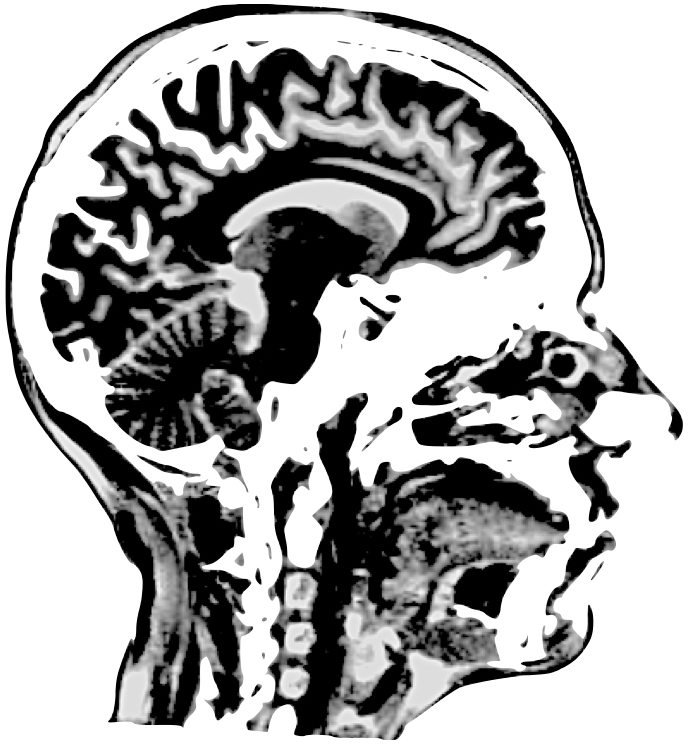
\includegraphics[scale=0.07]{brain}
}


\end{flushleft}
\end{minipage}
%%%%%%%%%%%%%%%%%%%%%%%%%%%%%%%%%%%%%%
%
%     Contact Info
%
%%%%%%%%%%%%%%%%%%%%%%%%%%%%%%%%%%%%%%
\hfill
\begin{minipage}[t]{0.35\textwidth}
\begin{flushleft}
\custombold{Email:} d-bridge@northwestern.edu \\
\custombold{Mobile:}  610.564.1589 \\
\links{
\custombold{Website:} \href{http://www.donnajobridge.com}{http://www.donnajobridge.com}  \\
\custombold{Professional:} \href{https://bit.ly/2FiAQVO}{https://bit.ly/2FiAQVO}
\custombold{GitHub:} \href{https://github.com/donnajobridge}{https://github.com/donnajobridge}
}
\end{flushleft}
\end{minipage}

%\noindent\makebox[\linewidth]{\color{headings}\rule{\paperwidth}{0.4pt}}
%\vspace{-15pt}

%{ \urlstyle{same}\url{http://debarghyadas.com}}
%\href{mailto:dd367@cornell.edu}{dd367@cornell.edu} | 607.379.5733

%\namesection{Peter B. Winter, Ph.D.}


%%%%%%%%%%%%%%%%%%%%%%%%%%%%%%%%%%%%%%
%
%     COLUMN ONE
%
%%%%%%%%%%%%%%%%%%%%%%%%%%%%%%%%%%%%%%

%%end of column 1
%%%%%%%%%%%%%%%%%%%%
% set size of column 1
\begin{minipage}[t]{0.65\textwidth}
\sectionsep
\sectionsep

\section{\underline{Objective}}
\sectionsep

\customboldB{I aim to join a team-oriented environment that tackles complex challenges \\using analytic and creative problem-solving} \\
\textbullet{} 10+ years creating high-quality research designs in data-intensive field \\
\textbullet{} End-to-end project implementation

%%%%%%%%%%%%%%%%%%%%%%%%%%%%%%%%%%%%%%
%     EXPERIENCE
%%%%%%%%%%%%%%%%%%%%%%%%%%%%%%%%%%%%%%
\sectionsep
\sectionsep
\section{\underline{Experience}}
\sectionsep
\runsubsection{Research Assistant Professor} \\
\descript{Northwestern University Feinberg School of Medicine \\  2015 - Present}

\sectionsep

\runsubsection{Cognitive Neuroscientist} \\
\descript{Northwestern University \\  2007 - Present}
\sectionsep
\location{Accomplishments}
\vspace{\topsep}
\begin{tightemize}
\item Developed independent line of research
\item 10+ peer-reviewed publications
\item 40+ conference presentations
\item Awarded 2 NIH grants totaling in > \$1 million in the past 2 years
\item Fully self-funded for 10 years (10 grants)
\end{tightemize}

\location{Human Subjects Research}
\begin{tightemize}
\item Conducted 30+ studies with 500+ in-person participants
\item Iteratively created and adapted interactive memory tasks for specific populations
\end{tightemize}


\location{Innovation}
\begin{tightemize}
\item Pioneered approach to merge 3+ data sources collected simultaneously
\item Developed technique using eye movements to predict memory \& brain activity 
\end{tightemize}


\location{Team Lead | Mentorship}
\begin{tightemize}
\item Led and managed teams of 3-6 people with diverse skill levels \& experience
\item Mentored and trained 5+ students/postdocs
\end{tightemize}


\location{Project + Program Management}
\begin{tightemize}
\item Cut through bureaucracies and navigated political landscapes to fulfill project goals
\item Managed and grew project budget 
\item Managed sensitive data and successfully met grant objectives
\end{tightemize}

\location{Clear Communication}
\begin{tightemize}
\item Delivered oral presentations to specialized audiences and general public
\item Conducted interviews with local and national media (NPR, LA Times, CNN, WTTW, Chicago Tonight)
\end{tightemize}


%%%%%%%%%%%%%%%%%%%%%%%%%%%%%%%%%%%%%%
%     Honors & Awards
%%%%%%%%%%%%%%%%%%%%%%%%%%%%%%%%%%%%%%
\sectionsep
\sectionsep
\section{\underline{Honors \& Awards}}
\sectionsep
\begin{description}[leftmargin=!,labelwidth=\widthof{\bfseries National Research and Service Award (NRSA Fellowship)}]
\item[National Research and Service Award (NRSA Fellowship)]  2014 – 2015
\item[Mechanisms of Aging and Dementia Fellowship] 2012 – 2014
\item[Human Cognition Fellowship]  2010 – 2012
\item[Cognitive Science Graduate Fellowship]  2009 – 2010
\item[Outstanding Research Achievement Award]  2006
\end{description}

%National Research and Service Award (NRSA Fellowship), Mechanisms of Aging and Dementia Fellowship,
%Human Cognition Fellowship, Cognitive Science Graduate Fellowship, Outstanding Research Achievement Award

\end{minipage} 
\hfill
\begin{minipage}[t]{0.3\textwidth} 

%%%%%%%%%%%%%%%%%%%%%%%%%%%%%%%%%%%%%%
%     SKILLS
%%%%%%%%%%%%%%%%%%%%%%%%%%%%%%%%%%%%%%


\sectionsep
\sectionsep

%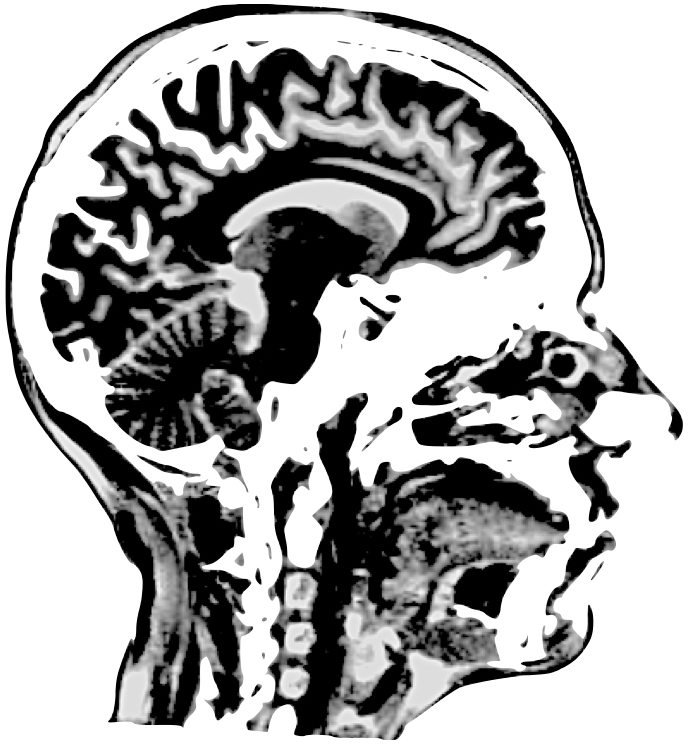
\includegraphics[scale=0.07]{brain}

\section{\underline{Skills}}
\sectionsep
\subsection{Data Analysis}
\location{Statistical Hypothesis Testing}
\textbullet{} \emph{t}-test, ANOVA, non-parametric, Monte Carlo methods \\
\sectionsep
\textbullet{} Data wrangling: 3D video, discrete events, time series
\sectionsep
 

\location{Feature Engineering}
\textbullet{} Finding quantifiable patterns in eye movements, behavior, and neural data \\
\sectionsep
 
\location{Time Series Analysis \& Signal Processing}
\textbullet{}  Regular \& irregular spacing, Fourier transform, wavelet convolution \\
\sectionsep
 

\location{Data Visualization}
\textbullet{}  Graphs and technical illustrations (Adobe Illustrator, MATLAB) \\
 
 \sectionsep
\sectionsep
\subsection{Programming}
\location{Computerized Memory Experiments}
\textbullet{}  Presentation Neurobehavioral Systems Inc. \\
\sectionsep
 

\location{Integrated Data Pipelines}
\textbullet{}  fMRI, EEG, behavior, and eye-tracking data \\
\sectionsep
\textbullet{}  MATLAB, FieldTrip, AFNI, EEGlab \\
\sectionsep
\textbullet{}  Python + Pandas \\

%%%%%%%%%%%%%%%%%%%%%%%%%%%%%%%%%%%%%%
%     Education
%%%%%%%%%%%%%%%%%%%%%%%%%%%%%%%%%%%%%%
\sectionsep
\sectionsep
\section{\underline{Education \& Training}}
\sectionsep
\location{Postdoctoral Fellow | \\
Cognitive Neuroscience } 
\begin{tightemize}
\sectionsep
\sectionsep
\item[] Northwestern University Feinberg School of Medicine, 2015
\end{tightemize}

\location{Ph.D. | Neuroscience } 
\begin{tightemize}
\item[] Northwestern University, 2012
\end{tightemize}

\location{B.A. | Women's Studies \& Psychology} 
\begin{tightemize}

\item[] Syracuse University, 2006
\end{tightemize}
\sectionsep


\begin{center}
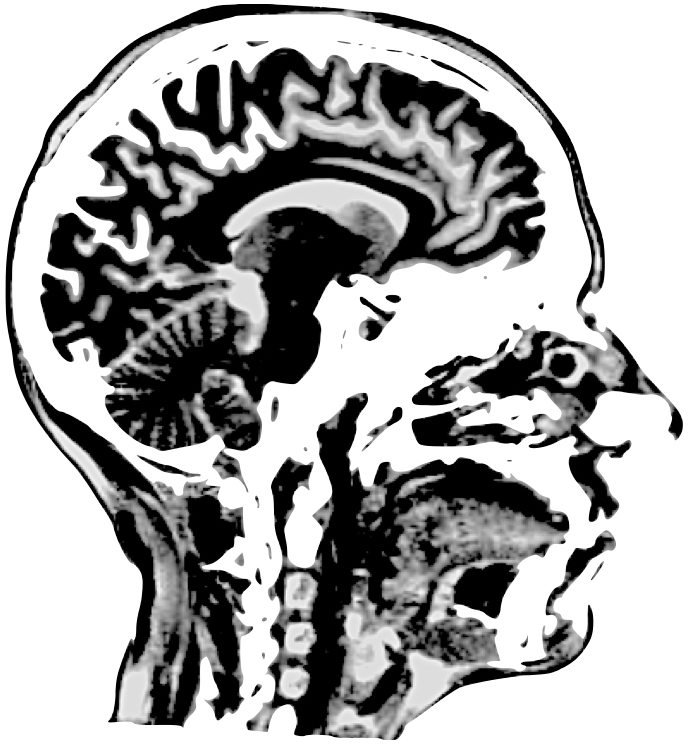
\includegraphics[scale=0.1]{brain}

\end{center}
\end{minipage} 



\end{document}  \documentclass[]{article}